\section{Vistas: Diagrama de Contexto}
En este diagrama se nos permite ver los diferentes agentes y las interacciones entre los mismos a alto nivel,
permitiendonos ademas, saber que agente controla las acciones y quien las monitorea.

Podremos observar que algunas de las interacciones descriptas en los escenarios se ven reflejadas en el diagrama, en el cual utilizamos los siguientes agentes:
\begin{itemize}
\item Gerente
\item PM 
\item Administrador (Admin) 
\item Cliente 
\item Proveedor
\item Subsistema de Mail 
\end{itemize}

\subsection{Diagrama general}
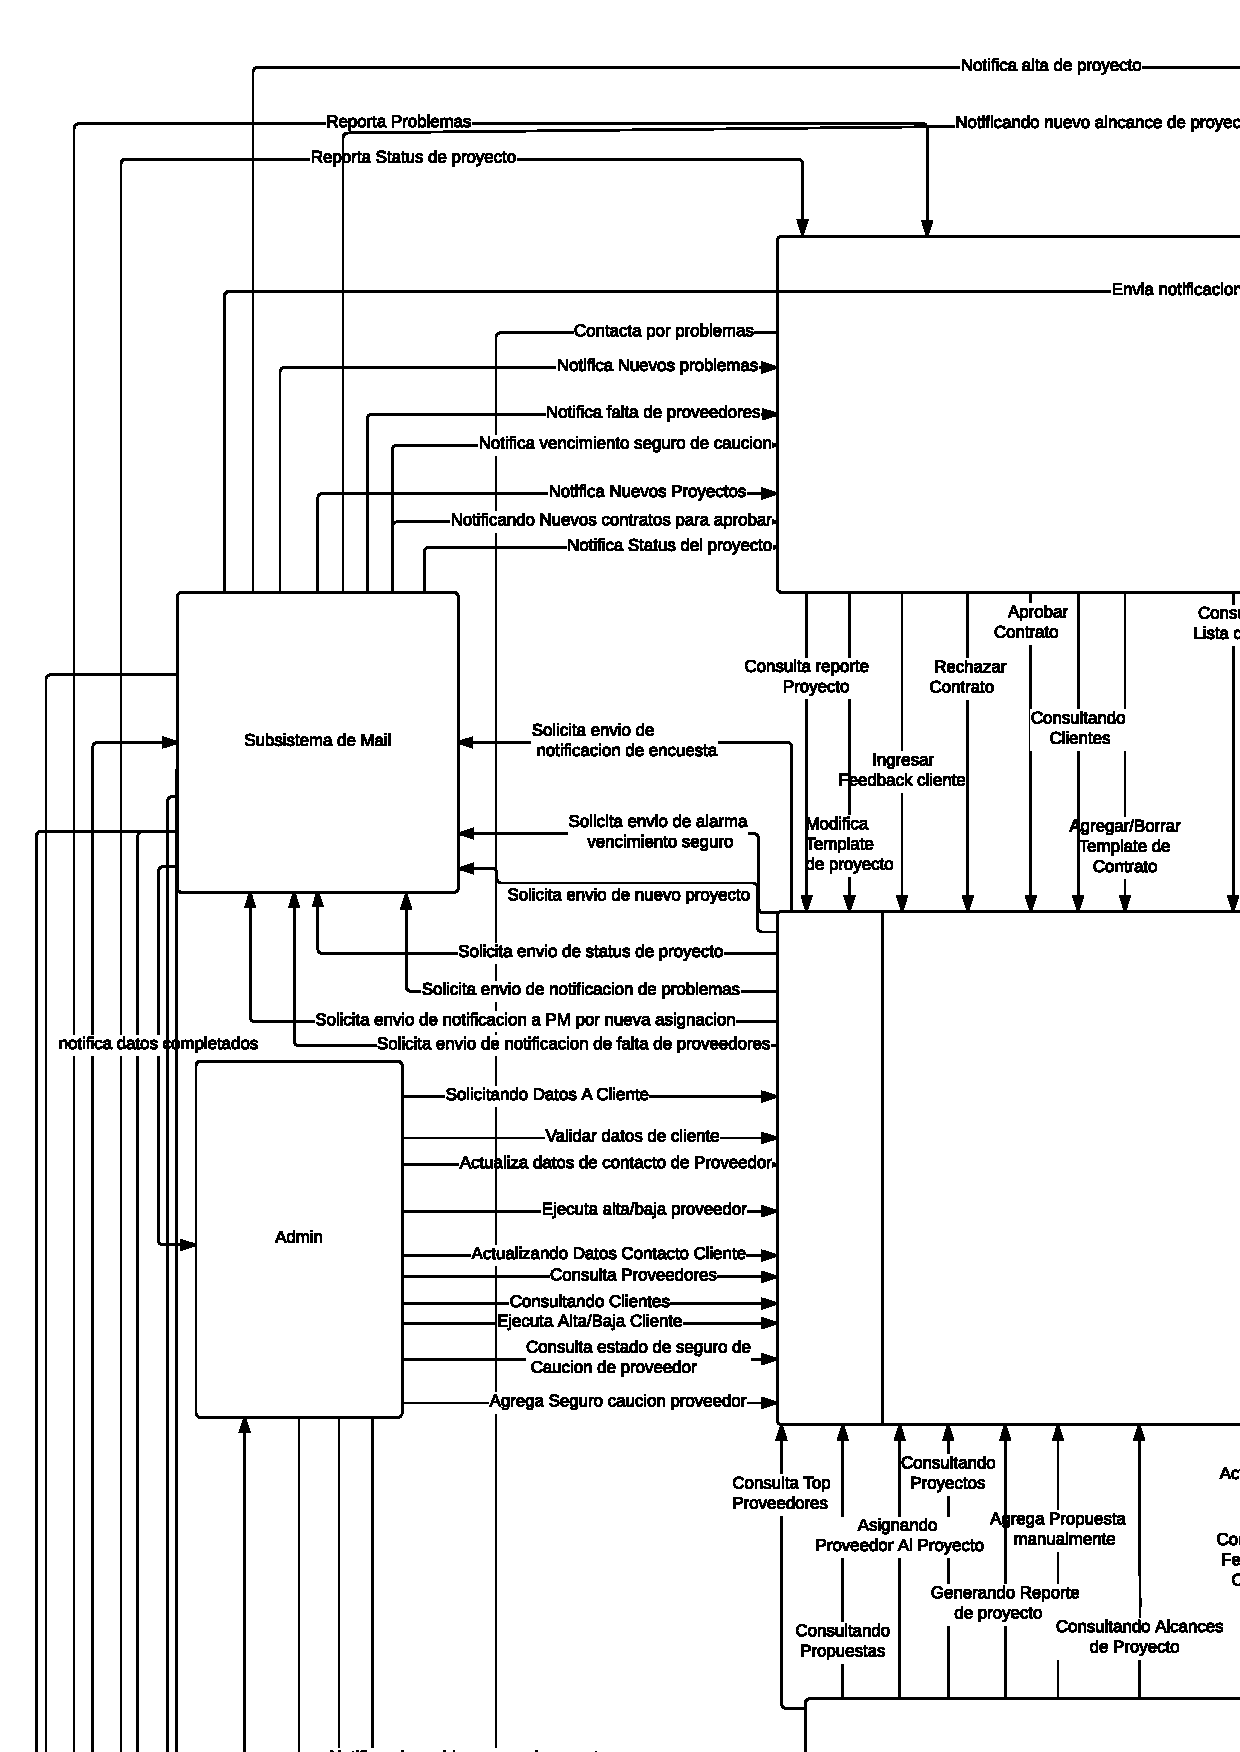
\includepdf[pages=-, offset=75 -75]{imagenes/contexto/contexto.pdf}
